% Figure 1: Problem 1 - fixed /24 per node vs buddy blocks (100 vs 500 pods)
% Same drawing as in ppt/project2/slides.tex. Compile: pdflatex fig1_problem1_fixed_vs_buddy.tex
\documentclass[border=4pt]{standalone}
\usepackage{amssymb}
\usepackage{tikz}
\usetikzlibrary{arrows.meta, positioning, fit, backgrounds, calc}
\renewcommand{\familydefault}{\sfdefault}
\tikzset{
  box/.style={draw, rounded corners, align=center, font=\scriptsize,
    minimum width=2.4cm, minimum height=0.6cm},
  arr/.style={-{Stealth[length=1.6mm]}, thick},
  biarr/.style={{Stealth[length=1.6mm]}-{Stealth[length=1.6mm]}, thick},
}
\begin{document}
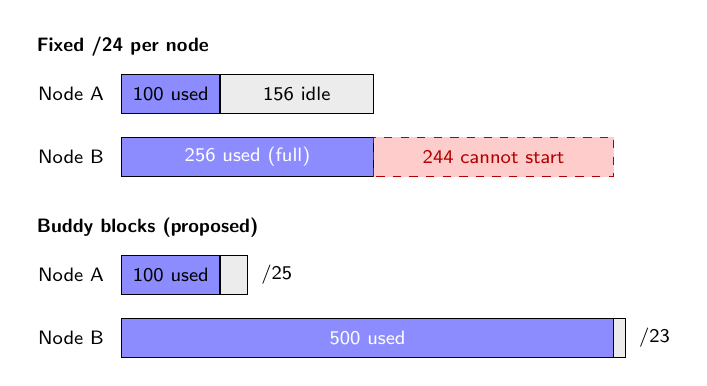
\begin{tikzpicture}[font=\scriptsize, x=1cm, y=1cm]
  \def\s{0.0125}
  \node[anchor=west, font=\scriptsize\bfseries] at (-1.2,1.0) {Fixed /24 per node};
  \node[anchor=east] at (-0.1,0.4) {Node A};
  \draw[fill=blue!45] (0,0.15) rectangle (100*\s,0.65);
  \draw[fill=gray!15] (100*\s,0.15) rectangle (256*\s,0.65);
  \node at (50*\s,0.4) {100 used};
  \node at (178*\s,0.4) {156 idle};
  \node[anchor=east] at (-0.1,-0.4) {Node B};
  \draw[fill=blue!45] (0,-0.65) rectangle (256*\s,-0.15);
  \node[text=white] at (128*\s,-0.4) {256 used (full)};
  \draw[fill=red!20, draw=red!70!black, dashed] (256*\s,-0.65) rectangle (500*\s,-0.15);
  \node[text=red!70!black] at (378*\s,-0.4) {244 cannot start};
  \node[anchor=west, font=\scriptsize\bfseries] at (-1.2,-1.3) {Buddy blocks (proposed)};
  \node[anchor=east] at (-0.1,-1.9) {Node A};
  \draw[fill=blue!45] (0,-2.15) rectangle (100*\s,-1.65);
  \draw[fill=gray!15] (100*\s,-2.15) rectangle (128*\s,-1.65);
  \node at (50*\s,-1.9) {100 used};
  \node[anchor=west] at (128*\s+0.05,-1.9) {/25};
  \node[anchor=east] at (-0.1,-2.7) {Node B};
  \draw[fill=blue!45] (0,-2.95) rectangle (500*\s,-2.45);
  \draw[fill=gray!15] (500*\s,-2.95) rectangle (512*\s,-2.45);
  \node[text=white] at (250*\s,-2.7) {500 used};
  \node[anchor=west] at (512*\s+0.05,-2.7) {/23};
\end{tikzpicture}
\end{document}
